\chapter{Etapas de preparación y ejecución de modelos}
\label{ch:method}

Inferir si una hipótesis brindará resultados positivos o negativos en un
proyecto de investigación es una de las tareas más complicadas de conocer con
antelación. Aún investigadores experimentados prueban decenas de ideas antes de
obtener algún descubrimiento concreto. Construir sistemas de aprendizaje
automático usualmente requieren de:

\begin{enumerate}
    \item Una hipótesis inicial la cual construir el sistema.
    \item Una implementación en algún lenguaje de programación.
    \item Ejecución de experimentos que permitan concluir si la idea original
    funciona de acuerdo a lo esperado.
\end{enumerate}

Basado en lo aprendido en esos 3 pasos, se vuelven a plantear nuevas ideas e
iterar sobre este proceso. Mientras más rápido se pueda finalizar un ciclo,
mayor será el progreso en la investigación. Debido a la larga lista de posibles
hipótesis para verificar, se deben obtener resultados prontamente, por lo
general, en a lo sumo una semana de haber iniciado el ciclo. Es por eso que una
prueba de concepto a partir de una implementación prototipo es más importante
que construir un sistema complejo en una etapa temprana de investigación.

No obstante, una vez validadas varias de las hipótesis, empezar nuevas
implementaciones a partir de los prototipos puede llegar a ralentizar el proceso
de desarrollo, ya que ciertos estándares de código no son tenidos en cuenta.
Tales como manejo de excepciones, documentación adecuada, o herramientas de
monitoreo y mantenimiento de código. El objetivo de estas pruebas de concepto es
la de otorgar experiencia a los investigadores para identificar los
requerimientos y resultados iniciales. Esto para luego construir un entorno de
desarrollo en esa dirección.

Durante las pruebas de concepto realizadas durante esta tesis se analizó la
factibilidad de la premisa inicial, encontrar un modelo de aprendizaje
automático a partir de una codificación de datos de planes relajados y acciones
etiquetadas que permitan guiar el proceso de grounding. Sin embargo, a medida
que el proyecto fue necesitando de experimentos más complejos, se agregaron
funcionalidades hasta construir un sistema de experimentación completo,
configurable, adecuado a nuestras necesidades, y que permita otorgar resultados
en el corto plazo de iniciado el ciclo de experimentación. Es por eso que en
este capítulo se describirán los detalles de implementación de cada uno de los
módulos que integran el flujo de ejecución de un experimento, abarcando el
dominio de planning utilizado, especificaciones de tareas STRIPS que se pueden
obtener a partir del dominio, persistencia de datos, preprocesamiento,
entrenamiento, evaluación de modelos, y registro y visualización de resultados.
Esto con el fin de describir los experimentos con mucha más claridad en el
capítulo \ref{ch:results}.
\section{Dominio de planning: Satellite}

\subsection{Descripción del dominio}

Para la construcción del conjunto de datos nos centramos en el dominio de
planning \emph{Satellite}, siendo parte del learninig track de la competencia
internacional de planning (IPC) del año 2011. Este dominio es un modelo del
problema de programación de observación satelital. Este implica el uso de uno o
más satélites para hacer observaciones, recopilar datos, y descenderlos a una
estación terrestre. Los satélites están equipados con diferentes instrumentos,
cada uno con características en términos de objetivos de calibración, producción
de datos, consumo de energía, y requisitos para el calentamiento y enfriamiento.
Los satélites pueden apuntar a diferentes objetivos con el fin de obtener
información de tal objeto. Existen restricciones sobre qué objetivos son
accesibles para un satélite debido a las capacidades de oclusión y rotación. Los
datos que generan los instrumentos de un satélite deben ser enviados a tierra
una vez ocurra una ventana de comunicación terrestre. La meta consiste en hallar
la cobertura (más eficiente) de las observaciones dadas las capacidades de los
satélites.

El cuadro \ref{tb:satellite_stats} resume los esquemas de acción del dominio con
su correspondiente tamaño de interfaz (Int), cantidad de precondiciones atómicas
(Pre), y cantidad de efectos atómicos (Eff). El Listing
\ref{lst:satellite-domain} muestra la especificación del dominio en PDDL.

\begin{table}[h!]
    \centering
    \scalebox{1}{
    \begin{tabular}{||c| c | c | c||} 
    \hline
    Esquema & Int & Pre & Eff\\ [0.5ex] \hline\hline
    %(take_image satellite0 planet5 instrument1 image1)
    take\_image & 4 & 6 & 1 \\ 
    calibrate & 3 & 4 & 1 \\ 
    turn\_to & 3 & 2 & 2 \\ 
    switch\_on & 2 & 2 & 3 \\ 
    switch\_off & 2 & 2 & 2 \\ [1ex] 
    \hline
    \end{tabular}}
    \caption{Ejemplos etiquetados a partir de un plan relajado y una acción}
    \label{tb:satellite_stats}
\end{table}

\begin{lstlisting}[
    float=!htb,
    caption={Dominio Satellite en PDDL.},
    label={lst:satellite-domain},
    language=PDDL]

    (define (domain satellite)
    (:requirements :strips :equality :typing)
    (:types satellite direction instrument mode)
    (:predicates 
             (on_board ?i - instrument ?s - satellite)
             (supports ?i - instrument ?m - mode)
             (pointing ?s - satellite ?d - direction)
             (power_avail ?s - satellite)
             (power_on ?i - instrument)
             (calibrated ?i - instrument)
             (have_image ?d - direction ?m - mode)
             (calibration_target ?i - instrument ?d - direction))
  
    (:action turn_to
     :parameters (?s - satellite ?d_new - direction ?d_prev - direction)
     :precondition (and (pointing ?s ?d_prev)
                        (not (= ?d_new ?d_prev)))
     :effect (and  (pointing ?s ?d_new)
                   (not (pointing ?s ?d_prev))))
   
    (:action switch_on
     :parameters (?i - instrument ?s - satellite)
     :precondition (and (on_board ?i ?s) 
                        (power_avail ?s))
     :effect (and (power_on ?i)
                  (not (calibrated ?i))
                  (not (power_avail ?s))))
   
    (:action switch_off
     :parameters (?i - instrument ?s - satellite)
     :precondition (and (on_board ?i ?s)
                        (power_on ?i))
     :effect (and (not (power_on ?i))
                  (power_avail ?s)))
  
    (:action calibrate
     :parameters (?s - satellite ?i - instrument ?d - direction)
     :precondition (and (on_board ?i ?s)
                        (calibration_target ?i ?d)
                        (pointing ?s ?d)
                        (power_on ?i))
     :effect (calibrated ?i))

    (:action take_image
     :parameters (?s - satellite ?d - direction ?i - instrument ?m - mode)
     :precondition (and (calibrated ?i)
                        (on_board ?i ?s)
                        (supports ?i ?m)
                        (power_on ?i)
                        (pointing ?s ?d)
                        (power_on ?i))
     :effect (have_image ?d ?m))
    )
\end{lstlisting}

\section{Manejo de datos}

\subsection{Generación de tareas de planning}
\label{method:data_generation}

Las instancias de problemas a partir del dominio Satellite se obtuvieron
automáticamente mediante un generador de problemas configurable de acuerdo a las
características que deseamos que tenga. Estas son la cantidad de satélites, la
cantidad máxima de instrumentos, el número de modos, el número de objetivos, y
el número de observaciones. A mayor sea algunos de estos parámetros, mayor el
número de acciones y facts necesarios para resolverlos. Una vez definida una
parametrización que represente las características de la tarea a modelar, el
generador devuelve su representación STRIPS especificada en PDDL.

% \url{https://github.com/AI-Planning/pddl-generators/tree/master/satellite}

Sean $\Pi^{PDDL} = (\mathcal{P}, \mathcal{A}, \Sigma^{C}, \Sigma^{O}, I, G)$ la
representación STRIPS en PDDL dada por el generador de problemas, y $\Pi = (F,
A, I, G)$ su tarea STRIPS asociada. La información que necesitamos recolectar
es:

\begin{enumerate}
    \item Un plan relajado $\vec{a}^{+}$ para $\Pi^{+}$.
    \item Un plan (en lo posible el óptimo) $\vec{a}$ para $\Pi$.
    \item El conjunto de objetos $\Sigma^{O}$.
    \item El conjunto de acciones instanciadas $A$ de $\Pi$.
\end{enumerate}

Los puntos 3, y 5 pueden obtenerse a partir de los archivos PDDL devueltos por
el generador. En cambio, 1, 2, y 4 requieren resolver la tarea por medio del
planificador de Fast Downward para ser obtenidos. Dado que $\Pi$ se obtiene a
partir de Fast Downward, el conjunto $A$ de acciones instanciadas contiene
únicamente aquellas que son alcanzables relajadamente desde el estado inicial
$I$. A su vez, en la medida de lo posible, se intentará obtener el plan óptimo
que resuelve $\Pi$. Esto se debe a la noción de relevancia de una acción para
resolver una tarea STRIPS. En un plan óptimo, las acciones que lo componen son
todas necesarias en la secuencia. Si una acción es eliminada, la secuencia
resultante no puede ser un plan de la tarea debido a que se obtendría un plan
con menos acciones que el plan óptimo y, por lo tanto, una contradicción (Lo cual
no es el caso para un plan genérico).

La información asociada a un problema obtenida por el generador y el
planificador se almacenan en directorios que contienen los siguientes archivos:

\begin{itemize}
    \item \emph{all\_operators.bz2}: Archivo comprimido del conjunto de acciones
    instanciadas.
    \item \emph{objects}: Conjunto de objetos del problema.
    \item \emph{problem.pddl}: Especificación en PDDL del problema.
    \item \emph{relaxed\_plan}: Plan relajado que resuelve la tarea relajada.
    \item \emph{optimal\_plan} o \emph{sas\_plan}: Plan (óptimo) que resuelve la
    tarea.
\end{itemize}

Por último, queda mencionar que tipo de problemas se generaron. Se dividieron en
3 grupos principales de acuerdo a su dificultad. 240 problemas a los cuales
pueden resolverse de manera óptima por el planificador, 48 a los cuales solo un
plan fue encontrado, y 18 que no pudieron resolverse debido a una falla en el
proceso de grounding. Es sobre este último grupo que nos interesa realizar
inferencia sobre las acciones que puedan ser relevantes para resolverlo y en los
que el modelo de aprendizaje automático debe guiar durante el proceso de
grounding. Es por eso que estos 25 problemas fueron elegidos para formar parte
de los problemas de test. Mientras que aquellos que sí logran resolverse (de
manera óptima o no) forman parte del material de entrenamiento.

Como veremos en la sección \ref{method:labeling}, requeriremos de los planes
reales para etiquetar estos datos y poder de esta forma realizar un análisis del
comportamiento del modelo. Por lo que es necesario encontrarles una solución a
los problemas de test. Afortunadamente, Satellite es uno de los dominios
trabajados en \citep{Gnad_Torralba_Dominguez_Areces_Bustos_2019} por lo que
limitaremos los problemas de test a aquellos problemas para los que una
solución fue hallada en este trabajo.

Otro inconveniente en los problemas de test, es la ausencia de las acciones
instanciadas para resolverlo. Aún habiendo logrado calcular un plan de la tarea,
la cantidad de instancias alcanzables relajadamente en $A$ es muy grande por la
cual no son dadas por el planificador al terminar el proceso de grounding, como
sí es el caso de los datos entrenamiento. Para resolver este problema, solo se generó
una muestra aleatoria de acciones instanciadas obtenidas a partir de grounding
cartesiano, por fuera del planificador.

Por lo tanto, tomaremos provecho de estas soluciones como una manera de
verificar que el modelo de aprendizaje logra desempeñarse correctamente antes de
probarlo en el planificador en tareas que no puedan instanciarse.

\subsection{Preservación de datos}

Una vez identificado qué problemas son utilizados como entrenamiento y cuáles como
test, es necesario preservar estos datos de manera organizada y de fácil acceso.
Si bien los datos se encuentran en archivos en una cierta estructura, no pueden
ser extraídos de manera programática. Por tal razón se tabularon y almacenaron
los datos en una base de datos relacional, para su posterior acceso por medio de
una herramienta de consultas.

Para el almacenamiento utilizamos una base de datos relacional de tipo SQL. La
figura \ref{fig:ERD} muestra su diagrama de entidad relación.

\begin{figure}[t!]
    \centering
    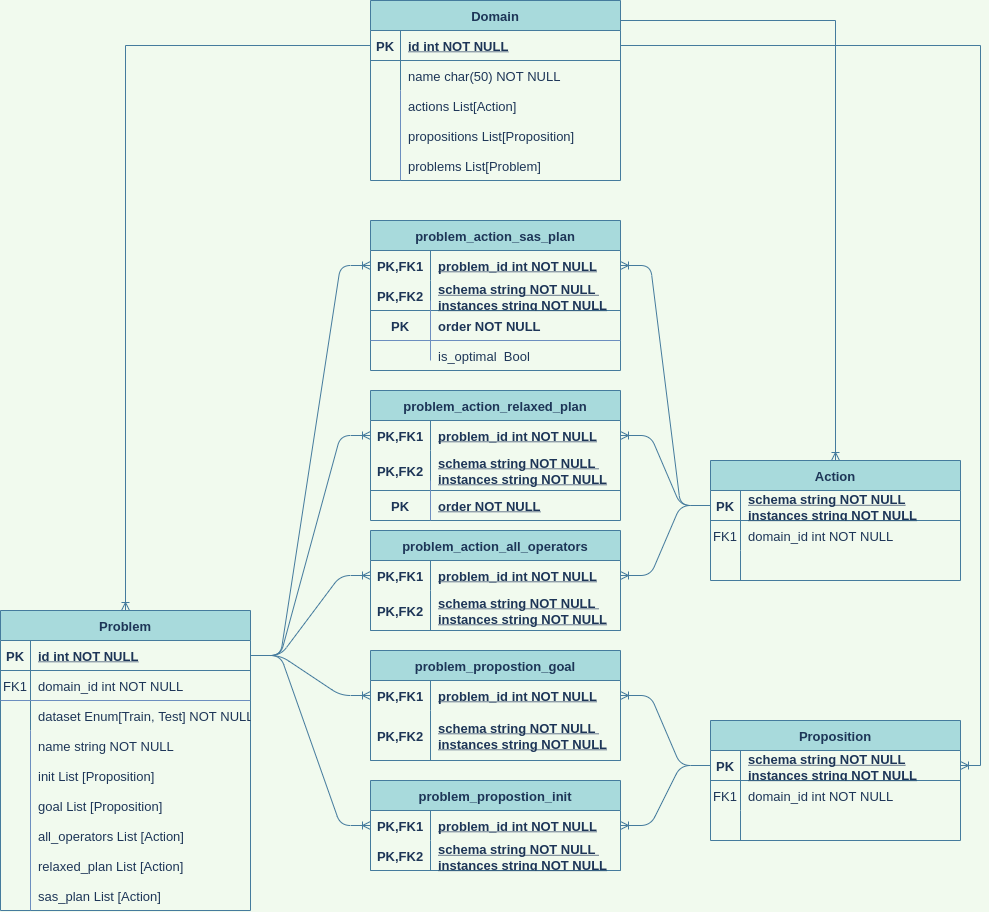
\includegraphics[width=\linewidth]{figures/ERD.png}
    \caption{Diagrama de entidad relación de la base de datos.}
    \label{fig:ERD}
\end{figure}

La tabla \emph{Problem} representa el conjunto de problemas. Algunas de sus
propiedades son, el nombre del problema (nombre dado por el generador), y el
conjunto al cual pertenece (entrenamiento o test). Para representar en la base
de datos tanto los planes relajados, como los planes que resuelven la tarea, se
utilizan relaciones \emph{many-to-many} a la tabla de acciones, manteniendo una
tabla intermedia que relaciona un problema con las acciones que conforman el
plan. Dado que las tablas en bases de datos relacionales se definen a partir de
la teoría de conjuntos, la repetición y el orden puede perderse para las
acciones que ocurren en un plan. Para resolver este problema se agregó el orden
de manera explícita como atributos en sus tablas. Ahora bien, notar que la tabla
\emph{Problem} tiene como atributos 2 listas, donde cada atributo representa de
manera ordenada (según algún criterio, en nuestro caso, el de los planes
relajados) los planes relajados, y los planes reales. Esto permite accederlos de
una manera mucho más práctica sin tener que utilizar el atributo del orden de
manera explícita al realizar una consulta. Para almacenar el conjunto de
acciones instanciables, el estado inicial, y la meta de un problema, simplemente
se utilaron otras tablas intermedias pero sin la necesidad de mantener el orden
esta vez.

Las tablas \emph{Action} y \emph{Proposition} almacenan todas las acciones y
facts instanciables relajadamente que hayan ocurrido en cualquier problema. Para
evitar repeticiones se agregó como clave primaria el nombre del esquema junto
con el de sus parámetros.

Por último, la tabla \emph{Domain} mantiene registro del dominio en caso de que
busquemos utilizar múltiples dominios además de Satellite en nuestros
experimentos.

Para realizar consultas a la base de datos empleamos un \emph{object relational
mapping} (ORM) que permite gestionar el acceso por medio de un lenguaje de
programación. El ORM considera cada tabla como una clase y elementos de la tabla
como objetos de tal clase. Por lo tanto, al efectuar una consulta el ORM mapea
los elementos partícipes de esa consulta a objetos del lenguaje de programación
Eso incluye cualquier otra relación u objeto que esté involucrado en la consulta
de manera directa o indirecta, cono es el caso del plan relajado, o el plan que
resuelve la tarea. De esta manera el ORM dispone al programador de todo el poder
de la programación orientada a objetos para manipular los datos.

\subsection{Etiquetado de ejemplos}
\label{method:labeling}

A partir de la base de datos es necesario generar una \emph{matriz de
entrenamiento} que será dada como entrada al modelo de aprendizaje automático.
En particular, mencionamos qué problemas se van a usar para entrenar los modelos
y cuáles para evaluarlos. Pero aún nos queda explicar cuál es la estructura
explicita de los pares $\{(\vect{x}_1, y_1), ..., (\vect{x}_n, y_n)\}$ de los
conjuntos de entrenamiento y test que recibirán como entrada los modelos
mencionados en el capítulo \ref{ch:lit_ml}.

Dado que buscamos aprender un modelo que prediga si una acción es relevante para
el plan real de un problema, necesitamos incluir en $\vect{x}$ información de
tal problema y la acción a cuál queramos averiguar su relevancia. Además, debe
ser fácil de calcular, tanto para las tareas de entrenamiento como las de test.
Como mencionamos en la sección \ref{lit:delete_relaxed}, para una tarea
especificada en PDDL, el planificador instancia el problema y realiza una
búsqueda exhaustiva guiada por medio de una función heurística definida usando
planes relajados. Si los planes relajados permiten guiar la búsqueda para
encontrar un plan de la tarea, entonces también podrían ser usados para guiar el
proceso de grounding. Por lo tanto, la estructura de los vectores de entrada
incluirán tanto el plan relajado como la acción que queremos estimar.

Por otro lado, en la sección \ref{method:data_generation} no sólo obtuvimos el
plan relajado de cada tarea generada, sino además el plan que lo resuelve junto
a las instancias de las acciones alcanzables relajadamente durante el proceso de
grounding. Por lo tanto, para una tarea en particular (y por ende un plan
relajado), se pueden identificar dos clases distintas de acciones generadas:

\begin{enumerate}
    \item Las acciones que pertenecen a la solución (óptima o no).
    \item Las acciones que no pertenece a la solución, pero que sí fueron
    generadas por el proceso de grounding por alcanzabilidad relajada de Fast
    Downward.
\end{enumerate}

A las acciones de 1 las denominamos \emph{good operators} de la tarea, y las de
2, \emph{bad operators} de la tarea. A estos dos conjuntos los denotaremos con
$A^{good}$ y $A^{bad}$ respectivamente.

\begin{algorithm}
    \caption{}\label{alg:training_data}
    \begin{algorithmic}
    \Require Plan relajado $\vec{a}^{+}$, $A^{good}$, y $A^{bad}$ de una tarea
    de la sección \ref{method:data_generation} \Ensure Matriz de ejemplos $M$ de
    tamaño $(|A^{good}| + |A^{bad}|) \times 3$ \State $M \gets [\ ]$ \For{$a \in
    A^{good} $} \State $M.push\_back((\vec{a}^{+}, a, 1))$ \EndFor
    
    \For{$a \in A^{bad} $} \State $M.push\_back((\vec{a}^{+}, a, 0))$ \EndFor
    
    \State \Return $M.to\_array()$
    \end{algorithmic}
\end{algorithm}

El algoritmo \ref{alg:training_data}, dado el plan relajado de un problema
y los conjuntos $A^{good}$ y $A^{bad}$, genera los datos etiquetados de una sola
tarea obteniendo una matriz como se muestra en el cuadro \ref{tb:matrix_shape}.

\begin{table}[h!]
\centering
\scalebox{0.9}{
 \begin{tabular}{||c | c | c||} 
 \hline
 Plan relajado & Acción & Etiqueta \\ [0.5ex] \hline\hline
 %(take_image satellite0 planet5 instrument1 image1)
 {}[switch\_on instrument0 satellite0, take\_image ...] & calibrate satellite0
 instrument0 star4 & 1 \\
 {}[switch\_on instrument0 satellite0, take\_image ...] & switch\_on instrument0
 satellite0 & 1 \\
 {}[switch\_on instrument0 satellite0, take\_image ...] & switch\_on instrument3
 satellite1 & 1  \\
 ... & ... & ...  \\
 {}[switch\_on instrument0 satellite0, take\_image ...] & turn\_to satellite0
 planet5 planet5 & 0 \\
 {}[switch\_on instrument0 satellite0, take\_image ...] & switch\_off
 instrument0 satellite0 & 0 \\
 {}[switch\_on instrument0 satellite0, take\_image ...] & switch\_on instrument3
 satellite1 & 0 \\ [1ex] 
 \hline
 \end{tabular}}
 \caption{Ejemplos etiquetados a partir de un plan relajado y una acción}
 \label{tb:matrix_shape}
\end{table}

La primera columna contienen una lista de acciones ordenadas y representan el
plan relajado de un problema, la segunda columna es la acción a consultar por su
relevancia, y la tercera columna es la etiqueta que indica si pertenece o no
al plan de la tarea.

Para generar los ejemplos de los problemas de entrenamiento y test, basta
con ejecutar el algoritmo \ref{alg:training_data} con cada uno de los problemas
uniendo las matrices resultantes.

Un inconveniente de esta representación es que la información del plan relajado
se multiplica $|A^{good}| + |A^{bad}|$ veces. Esto por cada terna plan relajado,
good operators, y bad operators. Veremos luego en la etapa de preprocesamiento
que el tamaño de la matriz además dependerá del largo de los planes relajados,
siendo una dificultad a superar durante los experimentos.

Por otro lado, notar que las matrices de los problemas de entrenamiento y de
test contienen información de todos los esquemas de acción de los problemas. En
la sección de experimentos veremos que nos interesará filtrar las filas por
esquemas de acción. Es decir, si tenemos un total de 5 esquemas en Satellite,
dividir la matriz del cuadro \ref{tb:matrix_shape} en 5 submatrices donde la
acción objetivo corresponda a un solo esquema.

Esto refleja una de las ventajas de haber utilizado una base de datos para
preservar la información. En lugar de almacenar los datos de todos los problemas
tanto de entrenamiento como de test ya etiquetados. Podemos realizar consultas
sobre información específica de los problemas haciendo consultas únicamente de
aquello que sea necesario para construir la matriz reduciendo de esta manera el
uso en memoria.

A partir de ahora, distinguiremos la noción de problemas de entrenamiento (test)
y conjunto de entrenamiento (test). Los problemas de entrenamiento (test) serán
aquellos que fueron separados en la sección \ref{method:data_generation},
mientras que el conjunto de entrenamiento (test) serán las matrices resultantes
de la forma del cuadro \ref{tb:matrix_shape} que se obtienen a partir de los
problemas.

\subsection{Preprocesamiento}
\label{method:preprocessing}

Como mencionamos en el capítulo \ref{ch:lit_ml} los conjuntos de entrenamiento y
de test deben ser codificados en algún valor numérico previamente a ser dados
como entrada a un modelo de aprendizaje automático. En particular, se trabajó con
dos tipos de codificación para representar los planes relajados y las acciones
de una tarea, una codificación ad-hoc basándonos en los métodos de tipo one-hot
y one-hot ordinal que describimos en la sección \ref{method:ohe}, y otra
codificación usando word embeddings descriptos en la sección \ref{method:wb}.

\subsubsection{Codificación ad-hoc de acciones y planes relajados}
\label{method:vectorization}

En la sección \ref{method:ohe} vimos que una de las codificaciones más sencillas
para una oración del lenguaje natural es por medio de una bolsa de palabras.
Podemos usar una idea similar para obtener una representación de los
planes relajados.

Tomemos una oración dada en el contexto de planning. La siguiente secuencia
muestra un plan relajado de largo 4 asociado a una tarea STRIPS, cuyos esquemas
de acción son \verb|calibrate|, \verb|switch_on|, \verb|take_image| y
\verb|turn_to|. El resto de las expresiones son objetos concretos del dominio.
También es importante mencionar que cada objeto de un cierto tipo está
enumerado. Por ejemplo el objeto \verb|instrument1| es del tipo
\verb|instrument| cuyo índice es $1$.

\begin{center}
    [\verb|calibrate satellite0 instrument1 groundstation0|, \\
    \verb|switch_on instrument1 satellite0|, \\
    \verb|take_image satellite0 planet5 instrument1 image1|, \\
    \verb|turn_to satellite0 groundstation0 planet5|] \\
\end{center}

La primera dificultad durante la codificación es decidir qué es una palabra de
la oración. Una posibilidad es definir cada acción como palabra y utilizar un
one hot encoding. Pero, por lo general una acción no suele ocurrir más de una
vez en un plan de la tarea, con lo que se perdería la información de la
frecuencia en que ocurren los objetos en la secuencia. Es clave capturar tanto
el tipo de los objetos como su índice. Por último, cada acción debe tener la
misma cantidad de componentes en su representación vectorial, independientemente
del esquema o el número de parámetros que reciba, y se debe asegurar el orden de
la secuencia.

Para resolver estas dificultades se definió la siguiente codificación ad-hoc:

\begin{itemize}
    \item Cada elemento en la interfaz de una acción junto a su esquema son
    definidos como palabras. Eso incluye la numeración de los objetos.
    \item Cada vector que representa a una acción tiene dimensión $2 \times N +
    1$ siendo $N$ la longitud de la interfaz más larga de un esquema. A aquellas
    acciones con una interfaz más chica se les agregará $0's$ hasta completar el
    largo requerido.
    \item Los esquemas de acción son enumerados en el rango $1, ..., M$, con $M$
    la cantidad de esquemas.
    \item El tipo de los objetos son enumerados en el rango de $1, ..., K$, con
    $K$ la cantidad de tipos.
    \item Si un objeto tiene el índice $i$ se lo incrementa en 1 (para evitar
    que aquellos objetos que tengan índice 0 se malinterpreten como márgenes).
\end{itemize}

Ejemplo: Dada la siguiente enumeración de esquemas de acción y tipos:

\begin{center}
    \{\verb|calibrate|: 1, \verb|turn_to|: 2, \verb|switch_on|: 3,
    \verb|take_image|: 4, \verb|switch_off|: 5\} \\
    \{\verb|satellite|: 1, \verb|instrument|: 2, \verb|planet|: 3,
    \verb|groundstation|: 4, \verb|image|: 5, \verb|star|: 6\}
\end{center}

Como la longitud de la interfaz más larga es 4, cada acción tendrá asociado un
vector de dimensión $2 \times 4 + 1 = 9$ y la codificación resultante sería la
siguiente:

\begin{table}[h!]
    \centering
    \begin{tabular}{l|c}
        \verb|calibrate satellite0 instrument1 groundstation0| & {} [1 1 1 2 2
        4 1 0 0] \\
        \verb|switch_on instrument1 satellite0| & {} [3 2 2 1 1 0 0 0 0] \\
        \verb|take_image satellite0 planet5 instrument1 image1| & {} [4 1 1 3 6
        2 2 5 2] \\
        \verb|turn_to satellite0 groundstation0 planet5| & {} [2 1 1 4 1 3 6 0
        0] \\
    \end{tabular}
\end{table}

Luego la codificación del plan relajado es la concatenación de los cuatro
vectores.

\begin{center}
    [1 1 1 2 2 4 1 0 0 3 2 2 1 1 0 0 0 0 4 1 1 3 6 2 2 5 2 2 1 1 4 1 3 6 0 0]
\end{center}

Por lo tanto, la matriz del cuadro \ref{tb:matrix_shape} estaría codificada de
la siguiente manera:

\begin{table}[h!]
\centering
\scalebox{0.9}{
 \begin{tabular}{||c | c | c||} 
 \hline
 Plan relajado & Acción & Etiqueta \\ [0.5ex] \hline\hline
 {}[3 2 1 1 1 0 0 0 0 4 ...] & {} [1 1 1 2 1 6 5 0 0] & 1 \\
 {}[3 2 1 1 1 0 0 0 0 4 ...] & {} [3 2 1 1 1 0 0 0 0] & 1 \\
 {}[3 2 1 1 1 0 0 0 0 4 ...] & {} [3 2 4 1 2 0 0 0 0] & 1  \\
 ... & ... & ...  \\
 {}[3 2 1 1 1 0 0 0 0 4 ...] & {} [2 1 1 7 6 7 6 0 0] & 0 \\
 {}[3 2 1 1 1 0 0 0 0 4 ...] & {} [5 2 1 1 1 0 0 0 0] & 0 \\
 {}[3 2 1 1 1 0 0 0 0 4 ...] & {} [3 2 4 1 2 0 0 0 0] & 0 \\ [1ex] 
 \hline
 \end{tabular}}
 \caption{Planes relajados y acciones etiquetadas usando codificación ad-hoc.}
 \label{tb:matrix_shape_ohe}
\end{table}

\subsubsection{Codificación por word embeddings de acciones y planes relajados}

Para esta codificación nuevamente surge la pregunta de qué consideramos una
palabra en un plan relajado. Para el caso de la codificación ad-hoc una palabra
estaba dada por cada una de las partes de una acción incluyendo la numeración de
los objetos. Para este caso, podríamos utilizar una interpretación similar para
las palabras, ya que cada una de esas componentes son parte importante de una
acción. Sin embargo, está vez optamos por considerar como una palabra al esquema
de acción y a las instancias de objetos en su interfaz, sin distinguir la
numeración como una palabra. El objetivo de esta decisión es intentar que el
modelo de word embeddings dependa por sí mismo, es decir, buscamos que dos
objetos del mismo tipo como \verb|satellite0| y \verb|satellite1| sean próximos
en la codificación.

Recordemos que los word embeddings tienen la propiedad de que palabras
semánticamente similares, son proyectadas cercas en un espacio N-dimensional.
Sin embargo, ¿Cuál es el significado de similitud en nuestro corpus de planes
relajados? ¿Cuál es el comportamiento que deseamos que aprenda el modelo del
lenguaje? Las propiedades que nos interesan capturar son:

\begin{enumerate}
    \item Las palabras de los esquemas de acción \verb|take_image|,
    \verb|turn_to|, \verb|calibrate|, \verb|switch_on|, \verb|switch_off|, y la
    de los objetos que las utilizan, sean proyectadas cerca en el espacio
    vectorial. Es decir, si \verb|switch_on| usualmente se instancia con los
    objetos de tipo \verb|instrument| y \verb|satellite|. Entonces las palabras
    \verb|switch_on|, \verb|instrumentX|, \verb|satelliteY| estén cerca
    vectorialmente para toda numeración de los objetos \verb|X|, \verb|Y|.
    \item En la codificación ad-hoc, distinguíamos la numeración de los objetos
    como una dimensión más en el espacio vectorial al cual proyectamos los
    datos. Como contraste, al utilizar word embeddings a nivel de
    subpalabras, buscamos que todos los objetos numerados de un mismo tipo se
    proyecten cerca en el espacio. Es decir, si consideramos el tipo
    \verb|instrument|, entonces para toda numeración \verb|X|, los vectores
    representación de \verb|instrumentX| están cerca.
    %Usualmente la numeración de los objetos en los problemas de test es mucho
    %mayor que en la de los de entrenamiento. Nos gustaría que el modelo de
    %lenguaje sea capaz de proyectar la numeración de los objetos en los planes
    %relajados de longitud más grande, a las vistas en los planes relajados de
    %entrenamiento. Ya que por lo general, a pesar de la cantidad de objetos en
    %los problemas de test, estos se suelen resolverse de manera similar a los
    %de entrenamiento. \textbf{TODO}: Consultar. Que buscamos que aprenda de la
    %numeración de los objetos? que dos palabras intrumentX, intrumentY esten
    %cerca para todo X, Y?
\end{enumerate}

Para capturar las propiedades 1 y 2 decidimos utilizar un modelo de lenguaje a
nivel de subpalabra (explicado en la sección \ref{method:wb_subwords}). En el
capítulo \ref{ch:results} uno de los objetivos será verificar que nuestras
suposiciones se cumplen para una parametrización concreta del modelo de
lenguaje.

La implementación utilizada del modelo de la sección \ref{method:wb_subwords} es
la de \emph{FastText} \citep{bojanowski-2017} desarrollada por \emph{Facebook}.
Para el entrenamiento, la implementación requiere como entrada un conjunto de
oraciones, en nuestro caso los planes relajados, separados por espacios para
distinguir sus palabras. Para distinguir una acción por sobre otra en la
secuencia, agregamos además 2 símbolos especiales, \verb|(| y \verb|)| al
comienzo y cierre de una acción. Por ejemplo para el plan relajado que mostramos
en la codificación ad-hoc

\begin{center}
    \verb|( calibrate satellite0 instrument1 groundstation0 )| \\
    \verb|( switch_on instrument1 satellite0 )| \\
    \verb|( take_image satellite0 planet5 instrument image1 )| \\
    \verb|( turn_to satellite0 groundstation0 plante5 )|
\end{center}

Esto se repitió para todos los planes relajados de los problemas de
entrenamiento, y se dio como entrada al modelo de FastText.

Una vez obtenido el modelo de lenguaje, conseguir la representación de una
acción y un plan relajado resulta sencillo. Solo es necesario proyectar cada una
de las partes que componen la acción o el plan relajado y calcular el promedio o
promedio normalizado (detallado en la sección \ref{lit:sentence_vector}) de
tales vectores. Por ejemplo si tenemos la acción:

\begin{center}
    \verb|calibrate satellite0 instrument1 groundstation0|    
\end{center}

Dividimos la oración en las palabras \verb|calibrate|,  \verb|satellite0|
\verb|instrument1| y \verb|groundstation0|. Entonces el vector de la oración es
obtenido como el promedio o promedio normalizado de los vectores de cada
palabra.

El caso de los planes relajados es similar. Supongamos que queremos codificar el
plan relajado anterior. Nuevamente separamos la oración en palabras (siendo
también un símbolo especial una palabra) y promediamos la representación de cada
una de ellas.

\begin{center}
\verb|(| \\
\verb|calibrate| \\
\verb|satellite0| \\
\verb|instrument1| \\
\verb|groundstation0| \\
\verb|)| \\
\verb|(| \\
\verb|take_image| \\
...
\end{center}

Por lo tanto, para un tamaño de 5 dimensiones para el vector de salida del
modelo de lenguaje, la matriz del cuadro \ref{tb:matrix_shape} estaría
codificada de la siguiente manera:

\begin{table}[h!]
\centering
\scalebox{0.9}{
 \begin{tabular}{||c | c | c||} 
 \hline
 Plan relajado & Acción & Etiqueta \\ [0.5ex] \hline\hline
 %(take_image satellite0 planet5 instrument1 image1)
 {}[0.1915,  0.0830,  0.2350, -0.0901,  0.0952] & {}[0.1674,
 0.0807,  0.1190, -0.0124,  0.0586] & 1 \\
 {}[0.1915,  0.0830,  0.2350, -0.0901,  0.0952] & {}[0.2077,
 0.0557,  0.0735, -0.0509,  0.0772] & 1 \\
 {}[0.1915,  0.0830, -0.2350, -0.0901,  0.0952] & {}[0.1797,
 0.0926,  0.1182,  -0.0022,  0.0544] & 1  \\
 ... & ... & ...  \\
 {}[0.1915,  0.0830,  0.2350, -0.0901,  0.0952] & {}[0.1694,
 0.0787,  0.1193,  -0.0063,  0.0626] & 0 \\
 {}[0.1915,  0.0830,  0.2350, -0.0901,  0.0952] & {}[0.1805,
 0.0261,  0.0897, -0.0131,  0.0651] & 0 \\
 {}[0.1915,  0.0830,  0.2350, -0.0901,  0.0952] & {}[0.1717,
 0.0793,  0.1258,  -0.0068,  0.0550] & 0 \\ [1ex] 
 \hline
 \end{tabular}}
 \caption{Ejemplos etiquetados a partir de un plan relajado y una acción}
 %\label{tb:matrix_shape}
\end{table}

Notar que la dimensión de los vectores del plan relajado y acción son las mismas
a diferencia de la codificación ad-hoc. En particular, para todo par de planes
relajados en la matriz, sus representaciones tienen la misma dimensión, lo cual
no ocurre para la codificación ad-hoc. Esto permite reducir enormemente la
dimensionalidad de los vectores que forman parte del conjunto de entrenamiento
como así también permite mantener la misma estructura y dimensión con el
conjunto de test. Lo cual es requerido por el clasificador que buscamos obtener.

\subsection{Generación de ventanas de planes relajados}

Mencionamos que el largo de los planes relajados de los problemas de
entrenamiento y de test varían. Lo cual para la codificación ad-hoc produce
vectores de planes relajados con dimensiones distintas. Esto no ocurre en la
codificación con word embeddings. Sin embargo, dado que el largo de los planes
relajados de test varía entre 250 a 500 acciones en comparación a los de
entrenamiento (Figura \ref{fig:plan-length-distplot}), realizar el promedio
puede generar que ciertas acciones de un esquema sean importantes, pero terminen
resultando opacadas por otro grupo con mayor frecuencia en la secuencia. Para
resolver estos problemas, los planes relajados de cada problema se partieron en
ventanas de contexto. En lugar de consultar sobre un plan relajado y una acción,
transformaremos los conjuntos de entrenamiento y de test a matrices compuestas por
ventanas de plan relajado y acción.

\begin{figure}[t!]
    \begin{subfigure}[b]{\textwidth}
        \centering
        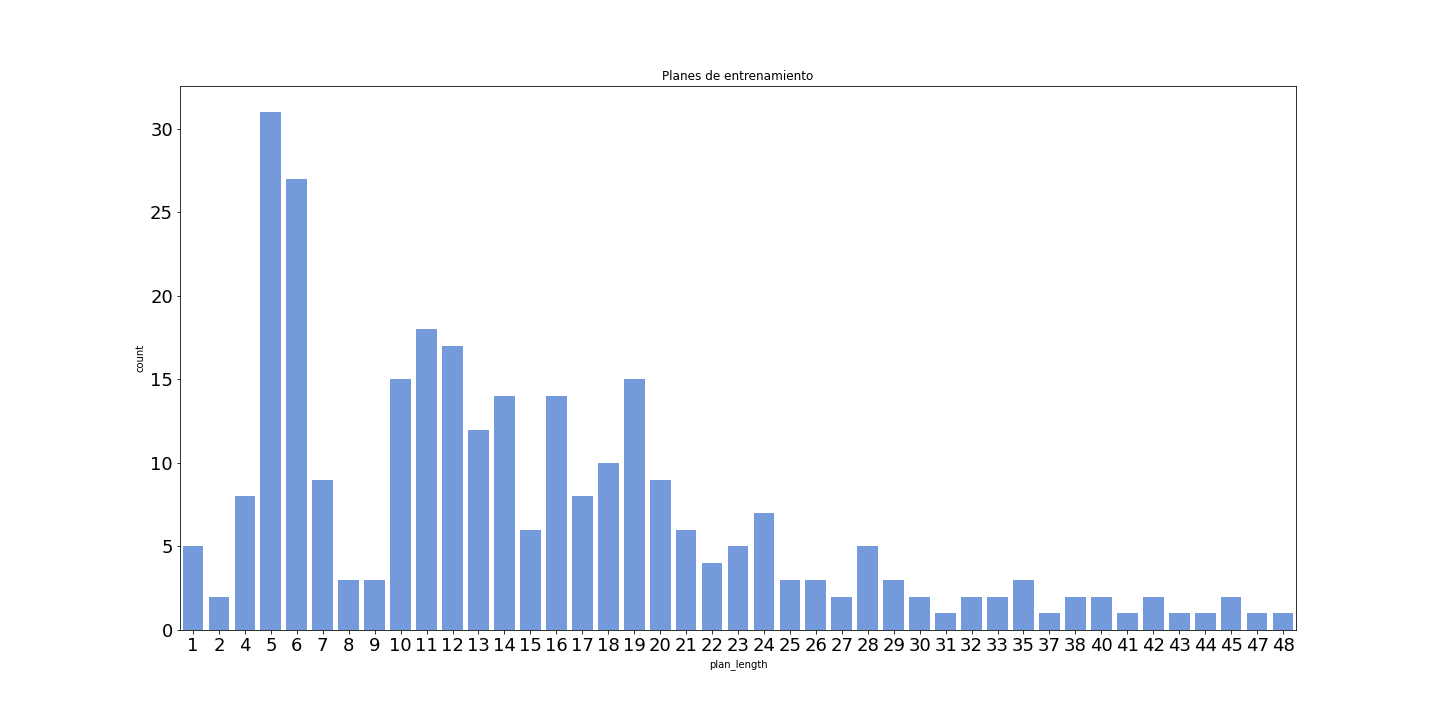
\includegraphics[width=\linewidth]{figures/plan_length_distplot_train.png}
        \caption{Planes relajados de entrenamiento}
        \label{fig:plan-length-distplot-train}
    \end{subfigure}
    \begin{subfigure}[b]{\textwidth}
        \centering
        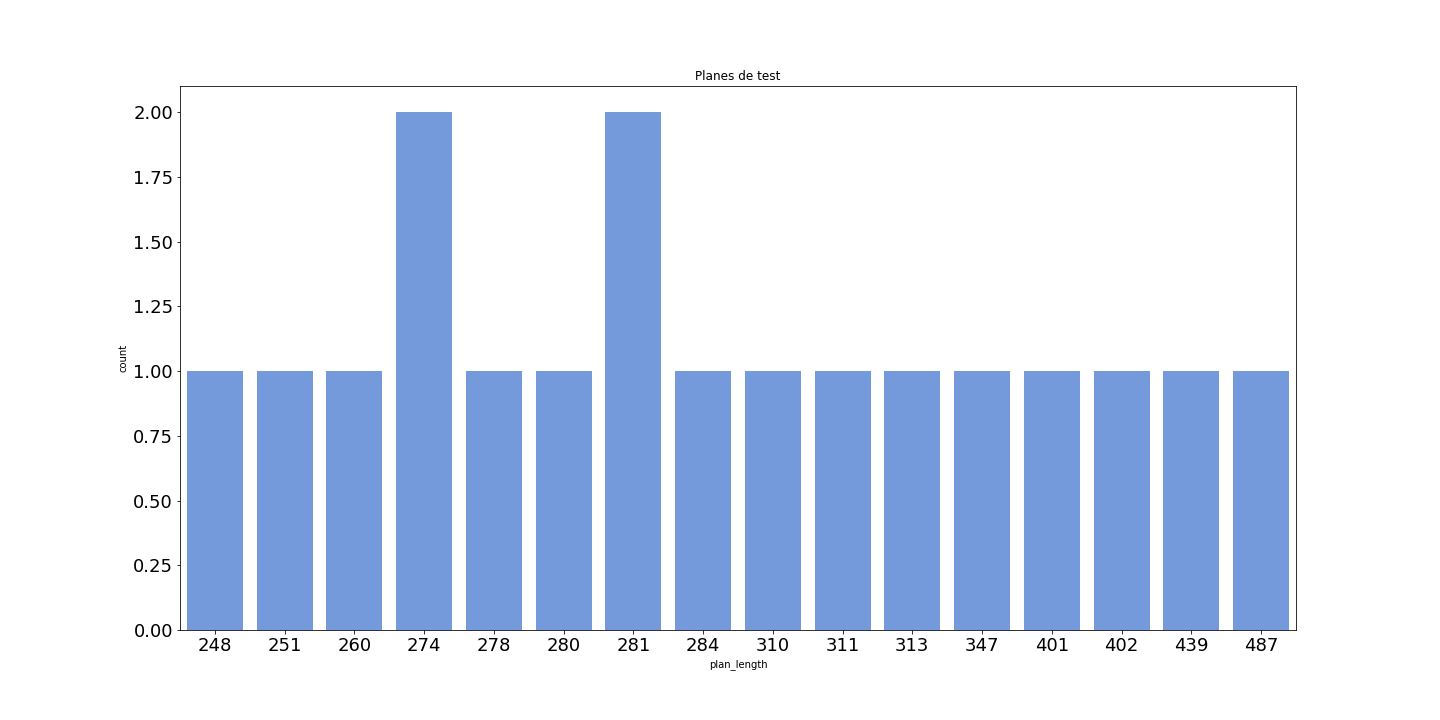
\includegraphics[width=\linewidth]{figures/plan_length_distplot_test.png}
        \caption{Planes relajados de test}
        \label{fig:plan-length-distplot-test}
    \end{subfigure}
    \caption{Distribución del largo de planes relajados}
    \label{fig:plan-length-distplot}
\end{figure}

La figura \ref{fig:window_example} muestra un ejemplo para una ventana de tamaño
3 y un paso de tamaño 2. Algo a notar de este ejemplo es que si la última
ventana generada no contiene la cantidad necesaria de acciones para generar una
ventana completa, se agregan palabras vacías hasta completar el largo restante.
Es importante también mencionar que ahora el tamaño de la matriz de entrenamiento
depende del largo de los planes relajados. En general, para una cantidad de
ventanas generadas $W$, good operators $N$, y bad operators $M$. Los ejemplos
generados son $W \times N \times M$. Por ejemplo, si para el plan relajado de la
figura \ref{fig:window_example}, se tienen 300 good operators y 1000 bad
operators. La cantidad de filas para ese problema es equivalente a $900000$
entradas. Esto es mucho peor para los problemas de test. Es por esto mismo que
no se pudieron generar muchos bad operators para estos problemas en la sección
\ref{method:data_generation}.

Una pregunta que queda por resolver es el valor de la etiqueta. Antes de incluir
las ventanas, nos interesaba determinar la probabilidad de que una acción sea
relevante para el plan real dado su plan relajado. Al utilizar las ventanas de
contexto, la pregunta es ligeramente distinta. Para este caso, nos interesa
determinar si la probabilidad de una acción es relevante para el plan real dada
una ventana del plan relajado. Si una acción es relevante en alguna ventana del
plan real entonces también lo es para el plan completo. Por lo tanto, para cada
uno de los planes relajados y acciones del conjunto de entrenamiento, propagamos
su etiqueta a su representación por partes.

\begin{figure}[t!]
    \centering
    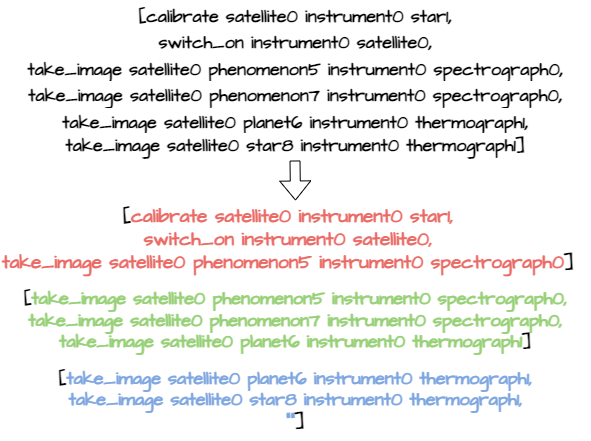
\includegraphics[width=\linewidth]{figures/window_example.png}
    \caption{Ejemplo de generación de ventanas para un plan relajado de largo 6.}
    \label{fig:window_example}
\end{figure}

Una vez generada las ventanas de planes relajados, obtenemos sus codificaciones
de manera ad-hoc o por word embeddings igual a como describimos en la sección
\ref{method:vectorization}.

\section{Selección de modelos}
\label{method:model_selection}

\subsection{Entrenamiento}

Una vez realizado el preprocesamiento estamos en condiciones de entrenar los
clasificadores que estudiamos en la sección \ref{lit:algorithms}. Los pares de
entrenamiento \{$(\vect{x}_1, y_1), ..., (\vect{x_n}, y_n)$\} para entrenar un
modelo de aprendizaje automático están compuestos por una representación de una
ventana perteneciente al plan relajado de un problema, y la representación de
una acción a estimar. Esto conforma el vector de características $\vect{x}_i$.
Las etiquetas reciben una codificación binaria de 1 o 0. Una etiqueta de 1
representa que la acción es relevante para el plan dado esa ventana del plan
relajado y una etiqueta de 0 indica lo contrario.

Para una configuración de parámetros, se entrena un clasificador utilizando
el conjunto de entrenamiento. A eso se agregan $k$ entrenamientos realizando
validación cruzada en $k$ grupos distintos. La única diferencia es que las
particiones son sobre los problemas de entrenamiento y no sobre el conjunto de
entrenamiento. Agrupar sobre este último puede llevar a que ventanas de un mismo
problema pertenezcan a grupos distintos y, por lo tanto, el problema esté
incompleto.

\subsection{Evaluación}

Una vez realizado los $k + 1$ entrenamientos del clasificador, deben ser
evaluados a partir del conjunto de test para obtener registro de las métricas
descriptas en la sección \ref{lit:metrics}. 

Inicialmente, es necesario generar las etiquetas, ventanas de planes relajados, y
codificación de los problemas de test. El conjunto de test resultante es dado
como entrada al modelo para obtener sus predicciones. Sin embargo, la evaluación
para nuestro problema es ligeramente distinta a la de un problema usual de
aprendizaje automático. Nuestro objetivo es estimar la probabilidad de que una
acción sea relevante para el plan real dado el plan relajado, pero el modelo
realizó sus predicciones a partir de ventanas del plan relajado. Es por eso que
la predicción final es la probabilidad máxima de todas las ventanas de un plan
relajado asociadas a una acción.

Ejemplo: Supongamos que tenemos la tabla de predicciones a nivel de ventanas de
plan relajado dado por la figura \ref{fig:window_example_evaluation}. Para la acción
\verb|switch on instrument0 satellite0|, la probabilidad máxima es la de la
ventana de color rojo. Por lo tanto, la predicción para esta acción dada el plan
relajado completo es la que predijo esa ventana.

\begin{figure}[t!]
    \centering
    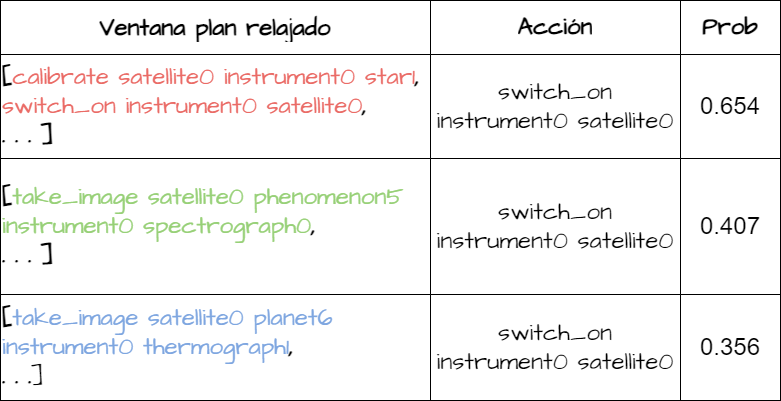
\includegraphics[width=\linewidth]{figures/aggregation_example.png}
    \caption{Ejemplo de evaluación por ventanas}
    \label{fig:window_example_evaluation}
\end{figure}

\section{Registro de resultados}

\subsection{Preservación de modelos, métricas, e imágenes}

Finalmente, evaluados los modelos, se almacenan los resultados (tanto métricas
como imágenes) de cada uno de los $k$ grupos, preservando únicamente los pesos y
parámetros del modelo entrenado con todo el conjunto de entrenamiento. Esto
último para aprovechar la totalidad de los ejemplos disponibles.

\subsection{Monitoreo y visualización}

Para el registro de métricas e imágenes se utilizó la librería \emph{MLFlow}.
 Esta herramienta permite el almacenamiento de datos y provee herramientas de
 visualización, registro de tiempos de ejecución de experimentos, comparación de
 experimentos, etc. Además de ser compatible con varias implementaciones de
 modelos. Algunas imágenes de las visualizaciones se pueden ver en la figura
 \ref{fig:mlflow-runs}.

 \begin{figure}[t!]
    \begin{subfigure}[b]{\textwidth}
        \centering
        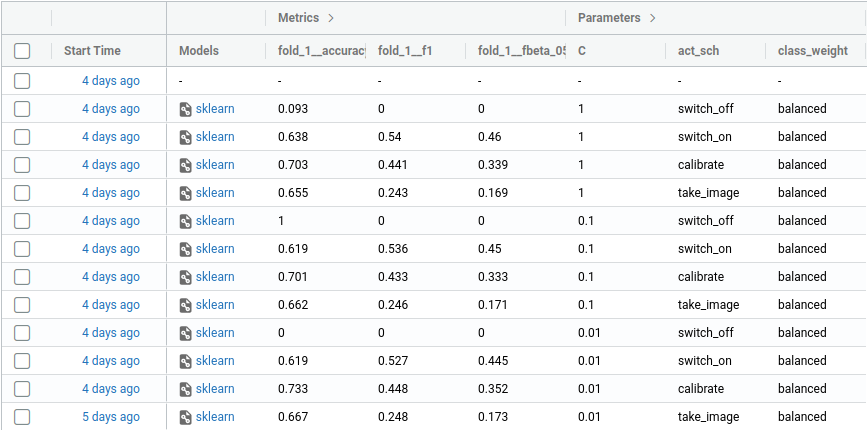
\includegraphics[width=\linewidth]{figures/runs_example_1.png}
        \caption{Tabla de resultados.}
    \end{subfigure}
    \hfill
    \begin{subfigure}[b]{\textwidth}
        \centering
        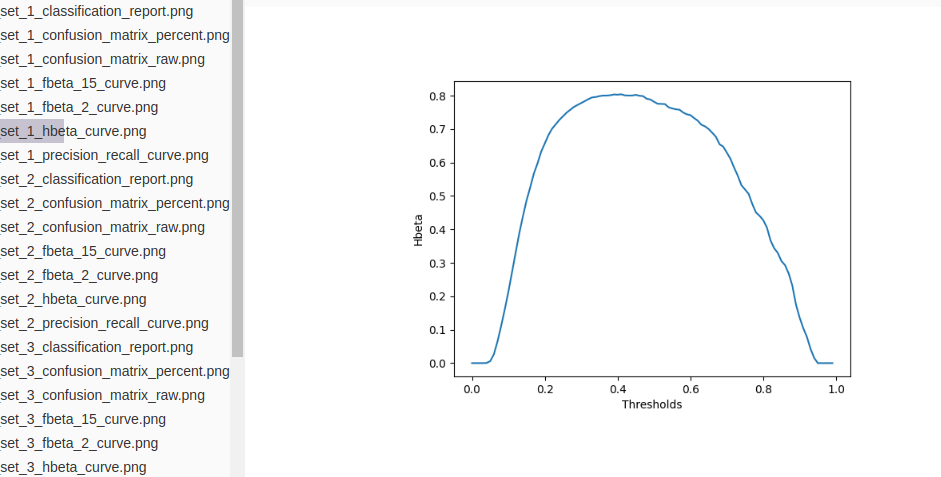
\includegraphics[width=\linewidth]{figures/runs_example_2.png}
        \caption{Visualización de gráficos.}
    \end{subfigure}
    \caption{Visualización de resultados desde MLFlow.}
    \label{fig:mlflow-runs}
\end{figure}

\subsection{Adaptación de modelos y transformadores}

En las secciones \ref{method:preprocessing}, y \ref{method:model_selection} se
puso mucho énfasis en la generación de los datos de esta tesis, así como los
pasos de exploración, preprocesamiento, entrenamiento y evaluación. Cada una de
estas etapas requirieron:

\begin{enumerate}
    \item Generación de especificaciones de problemas del dominio Satellite.
    \item Extracción de planes relajados, acciones instanciadas, y soluciones de
    los problemas a partir del planificador de Fast Downward.
    \item Separación en problemas de entrenamiento y test.
    \item Almacenamiento y preservación en una base de datos.
    \item Generación de conjuntos de entrenamiento y test.
    \item Transformación de los conjuntos de entrenamiento utilizando ventanas
    de planes relajados.
    \item Codificación de ventanas y acciones.
    \item Entrenamiento.
    \item Evaluación.
    \item Registro de resultados.
\end{enumerate}

Para la implementación de estos pasos se utilizó como lenguaje de programación
\emph{Python}. No obstante las librerías y herramientas principales requirieron
ser adaptadas a una interfaz común de tal manera que puedan ejecutarse de manera
sistemática. Esto se debió a que cada herramienta sigue sus propias convenciones.
Por ejemplo, la extracción de datos y lectura de archivos necesitó de librerías
que trabajen sobre el sistema de archivos, la persistencia de datos fue por
medio de \emph{SQL}, las consultas de bases de datos fueron realizadas por medio
del ORM \emph{SqlAlchemy}, las etapas de preprocesamiento en mayor parte fueron
con herramientas de \emph{Numpy} y \emph{Pandas}. La regresión logística y
XGBoost proveían una interfaz a través de \emph{Scikit-learn}, pero las redes
neuronales fueron implementadas en \emph{Pytorch}. La validación cruzada,
evaluación, y obtención de métricas también se hicieron con \emph{Scikit-learn}.
Y el registro de datos con \emph{MLflow}. Al momento de usar estas librerías
claramente fue necesario implementar una interfaz en común que minimice su
acoplamiento, este fue también uno de los desafíos de este trabajo.